\documentclass[border=3pt]{standalone}
% Preâmbulo compartilhado pelos diagramas TikZ da aula 13 (SLAM com EKF)
\usepackage[T1]{fontenc}
\usepackage[utf8]{inputenc}
\usepackage{lmodern}
\usepackage{amsmath}
\usepackage{xcolor}
\usepackage{tikz}
\usetikzlibrary{arrows.meta,angles,quotes,decorations.pathmorphing,decorations.pathreplacing,calc,
                positioning,shapes.geometric,shapes.misc,backgrounds,fit,
                math}

% Paleta (mesma dos SVGs originais)
\definecolor{dblue}{HTML}{2A5B8C}
\definecolor{dorange}{HTML}{B3541E}
\definecolor{dgreen}{HTML}{4A7C59}
\definecolor{dred}{HTML}{9C4B4B}
\definecolor{dcream}{HTML}{F4F1EA}
\definecolor{dshade}{HTML}{DDD7C9}

% Função gaussiana (não normalizada por padrão de escala visual)
\pgfmathdeclarefunction{gauss}{3}{%
  \pgfmathparse{1/(#3*sqrt(2*pi))*exp(-((#1-#2)^2)/(2*#3^2))}%
}

% Estilos comuns (prefixo d... para não colidir com chaves internas do pgf)
\tikzset{
  >={Stealth[length=2mm]},
  dguide/.style={gray!55, dashed, line width=0.4pt},
  daxis/.style={gray!60, line width=0.7pt, ->},
  dbody/.style={fill=black!3, draw=black!80, line width=1pt},
  dacc/.style={draw=dblue, line width=1pt},
  dlbl/.style={black!55, font=\small},
  dsub/.style={black!45, font=\footnotesize},
  dstate/.style={circle, draw=black!80, fill=dcream, line width=1pt,
                 minimum size=17mm, font=\large, inner sep=1pt},
  dobs/.style={circle, draw=black!80, fill=dshade, line width=1pt,
               minimum size=14mm, font=\large, inner sep=1pt},
  dbox/.style={rounded corners=2pt, draw=black!80, fill=dcream, line width=1pt,
               align=center, inner sep=6pt},
  dop/.style={circle, draw=black!80, fill=white, line width=1pt,
              minimum size=6mm, inner sep=0pt, font=\small},
  dtrans/.style={->, dblue, line width=1pt},
  dmeas/.style={->, dorange, line width=1pt},
  dcurve/.style={line width=1pt, dblue},
  dcurveb/.style={line width=1.4pt, dorange},
}

\begin{document}
\hyphenpenalty=10000 \exhyphenpenalty=10000 \tolerance=9999 \emergencystretch=3em
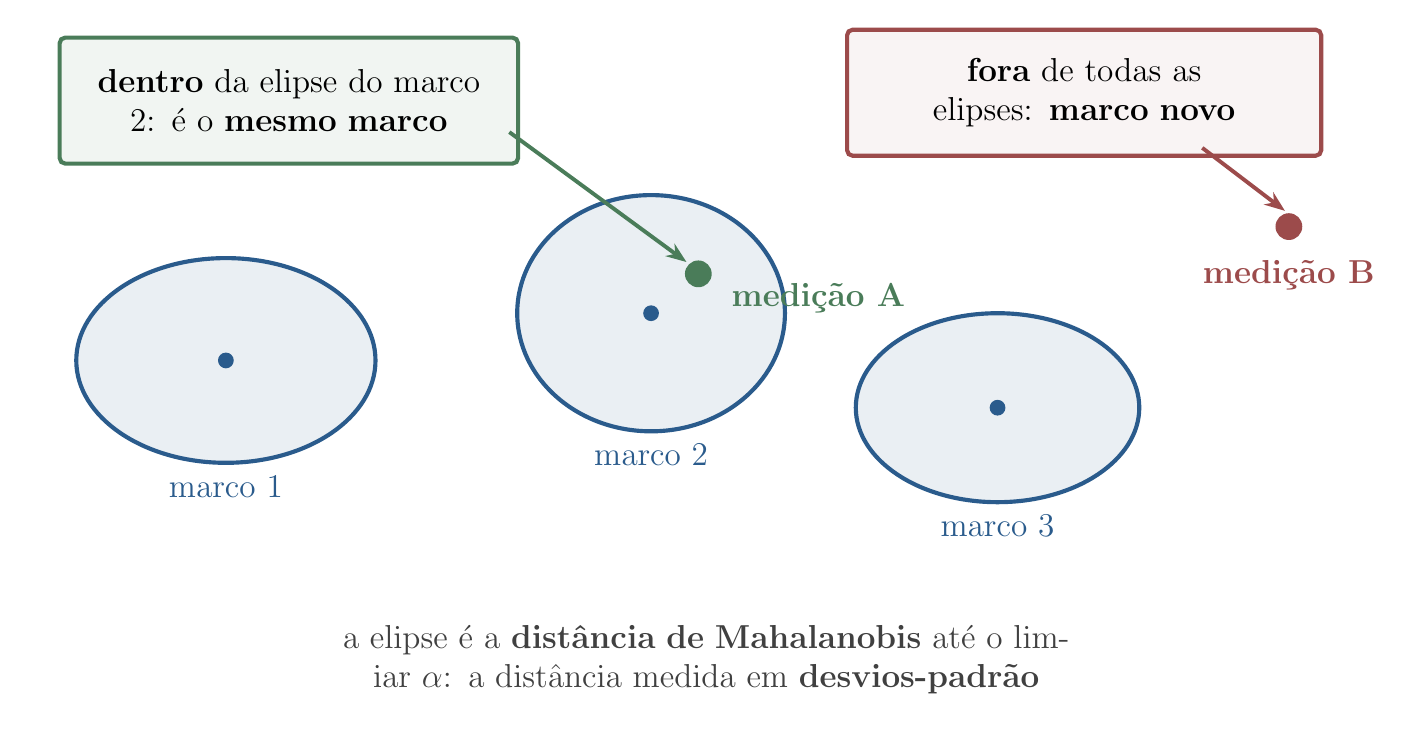
\begin{tikzpicture}[x=1cm,y=1cm]
\tikzset{e/.style={dblue, fill=dblue!10, line width=1.5pt}}
\draw[e] (3.4,4.6) ellipse (1.9 and 1.3); \fill[dblue] (3.4,4.6) circle (0.1); \node[font=\large, dblue] at (3.4,3.0) {marco 1};
\draw[e] (8.8,5.2) ellipse (1.7 and 1.5); \fill[dblue] (8.8,5.2) circle (0.1); \node[font=\large, dblue] at (8.8,3.4) {marco 2};
\draw[e] (13.2,4.0) ellipse (1.8 and 1.2); \fill[dblue] (13.2,4.0) circle (0.1); \node[font=\large, dblue] at (13.2,2.5) {marco 3};
\fill[dgreen] (9.4,5.7) circle (0.17); \node[font=\large\bfseries, dgreen, anchor=west] at (9.7,5.4) {medição A};
\fill[dred] (16.9,6.3) circle (0.17); \node[font=\large\bfseries, dred, anchor=north] at (16.9,6.0) {medição B};
\node[dbox, draw=dgreen, fill=dgreen!8, line width=1.5pt, text width=5.4cm, minimum height=1.6cm, font=\large] at (4.2,7.9) {\textbf{dentro} da elipse do marco 2: é o \textbf{mesmo marco}};
\node[dbox, draw=dred, fill=dred!6, line width=1.5pt, text width=5.6cm, minimum height=1.6cm, font=\large] at (14.3,8.0) {\textbf{fora} de todas as elipses: \textbf{marco novo}};
\draw[dgreen, line width=1.4pt, -{Stealth[length=2.6mm]}] (7.0,7.5) -- (9.25,5.85);
\draw[dred, line width=1.4pt, -{Stealth[length=2.6mm]}] (15.8,7.3) -- (16.85,6.5);
\node[font=\large, black!75, text width=17cm, align=center] at (9.5,0.8) {a elipse é a \textbf{distância de Mahalanobis} até o limiar $\alpha$: a distância medida em \textbf{desvios-padrão}};
\end{tikzpicture}
\end{document}
